\section{Implementation}
Development of OSM started with development in phases which focus on particular need of project.
Various phases and their detail are given below -:
\begin{itemize}
\item Phase I (Setup OSM Server) -: \\
        During Phase I, install all the dependecies(components) as mentioned above to make your own osm tile sever. After installing the softwares download the map in pbf(may be osm) format and render your own tile server. You can see your map on the browser after moving to the location which is being downloaded.

\begin{figure}[h!]
\centering 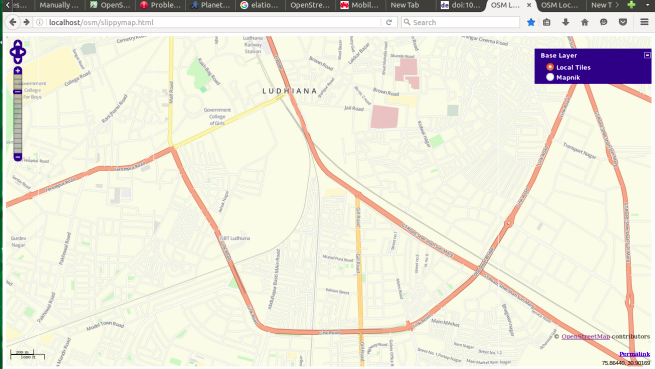
\includegraphics[width=0.7\textwidth]{input/images/osm7.png}
\caption{OSM Map on Web browser}
\end{figure}

\item Phase II (Styling of Map) -: \\
        During phase II, there is a lot of customization as listed below:-
\begin{itemize}
\item Colors of the buildings, roads, primary lines, secondary lines etc have been customized and then re-render the map to view the changes in the map.
\begin{figure}[h!]
\centering 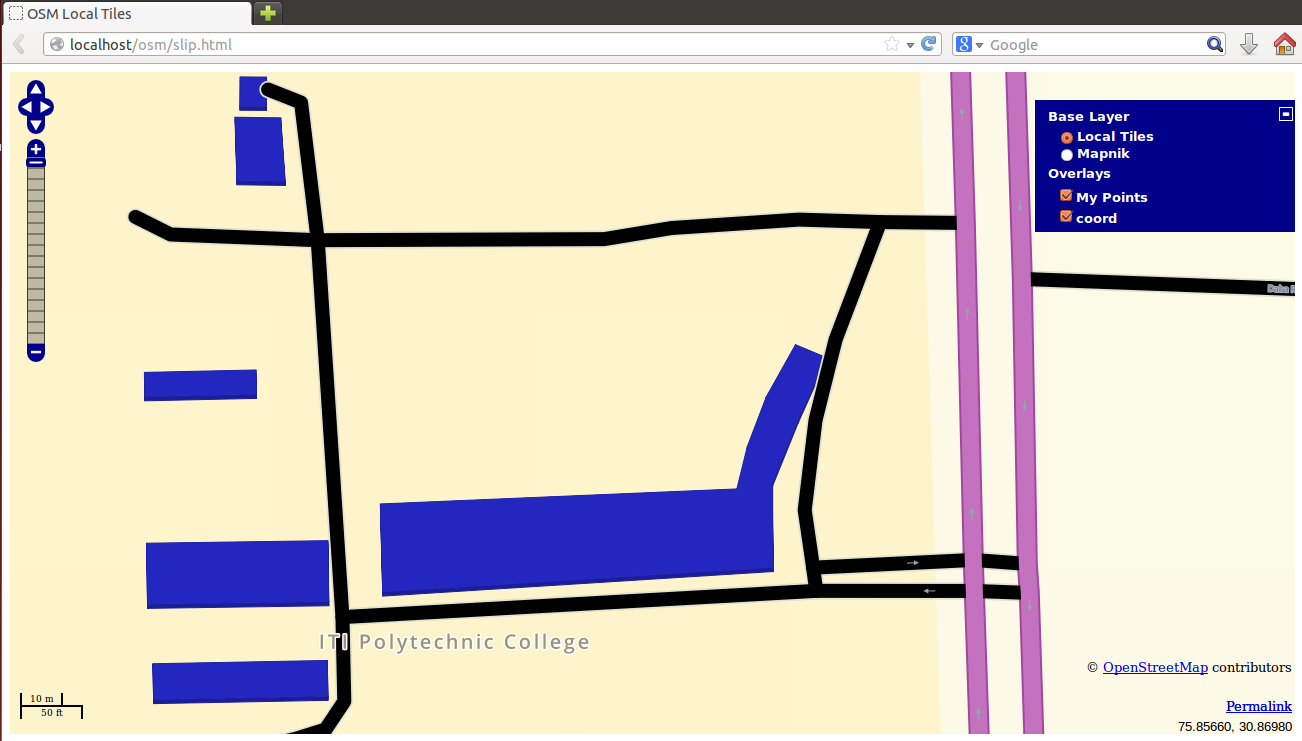
\includegraphics[width=0.7\textwidth]{input/images/osm5.png}
\caption{Building with customize color}
\end{figure}

\item Added international boundary of India with customizable color and pixels.
\begin{figure}[h!]
	\centering 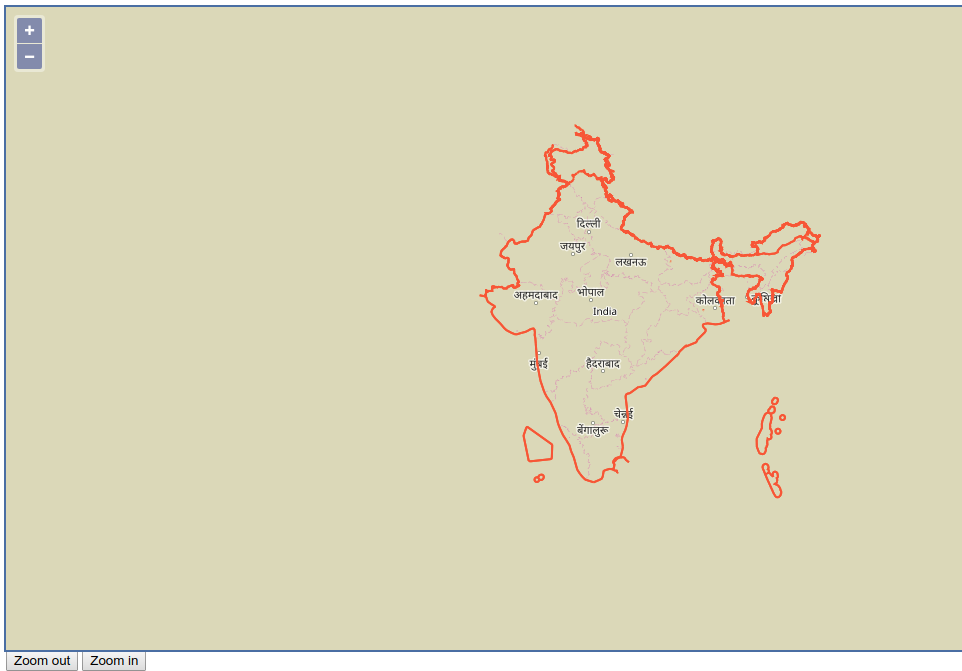
\includegraphics[width=0.7\textwidth]{input/images/osm_boundary.png}
	\caption{International Boundary of India}
\end{figure}

\item Modified the icons of the nodes.
\begin{figure}[h!]
	\centering 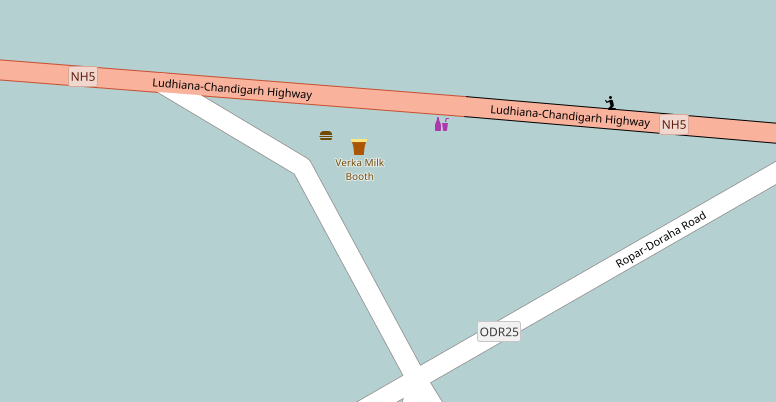
\includegraphics[width=0.7\textwidth]{input/images/osm_icon.png}
	\caption{Customized icon representing Pub shop}
\end{figure}

\item Customize the language of the map by applying Algorithm- if Punjabi name is provided then first priority goes to it followed by hindi and then English.
\begin{figure}[h!]
	\centering 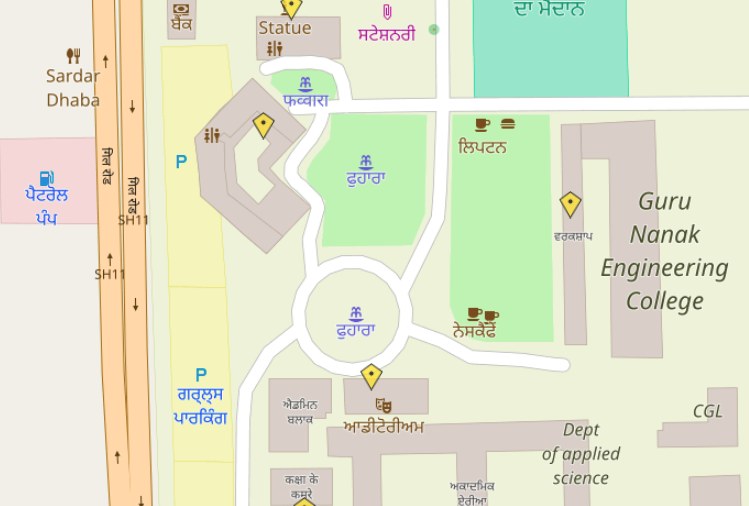
\includegraphics[width=0.7\textwidth]{input/images/osm_language.png}
	\caption{Map of Punjab in Punjabi}
\end{figure}

\item Admin levels at different zoom levels with different colors and with a names displayed over each boundary area.	
	\begin{figure}[h!]
		\centering 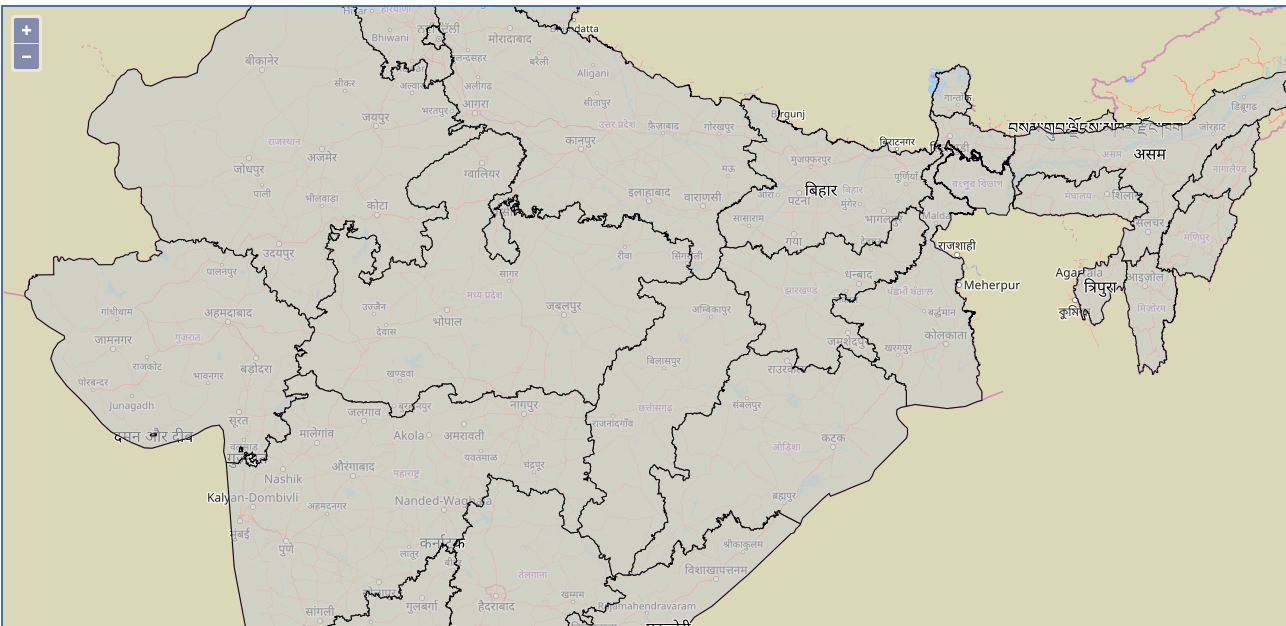
\includegraphics[width=0.7\textwidth]{input/images/osm_level_4.png}
		\caption{India divided into states with different color}
	\end{figure}

	\begin{figure}[h!]
	         \centering 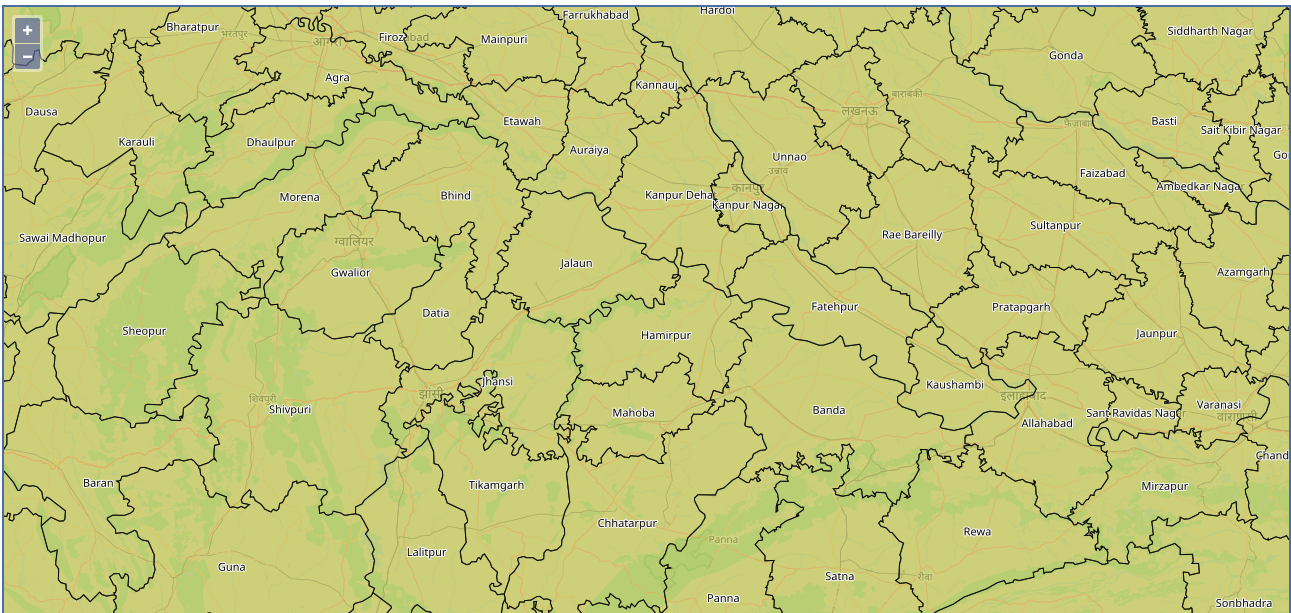
\includegraphics[width=0.7\textwidth]{input/images/osm_level8.png}
                 \caption{India divided into districts with different color}
	\end{figure}

\end{itemize}
\item Phase III (Increased zoom levels to 28 for indoor mapping) -: \\
	        The purpose of phase III was to increase the zoom levels to more than 19 so to create the space for indoor mapping. It is done in mod\_tile module by applying another different algorithm. 
		\begin{figure}[h!]
			\centering 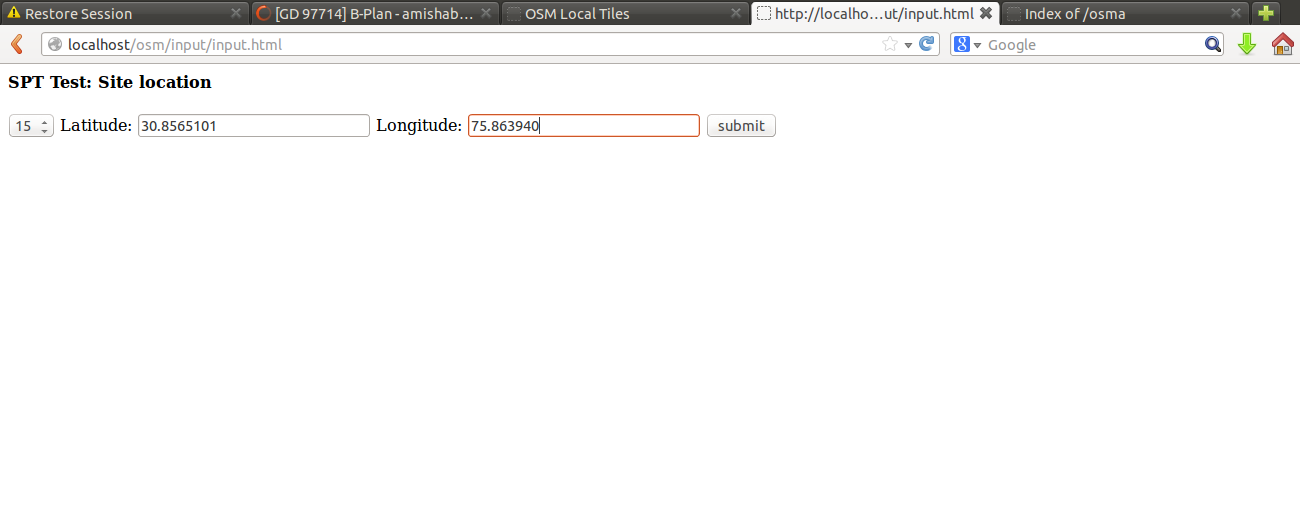
\includegraphics[width=0.7\textwidth]{input/images/osm2.png}
			\caption{Increased zoom level for indoor mapping}
		\end{figure}

\item Phase IV (User Input Map) -: \\
        During phase III, we made the html and php pages in which user can input latitude, longitude and zoom level of his own choice and if the tile image of that location is downloaded then on one click the map of that particular location will be visible. The functioning is done with the help of Javascript.
\begin{figure}[h!]
\centering 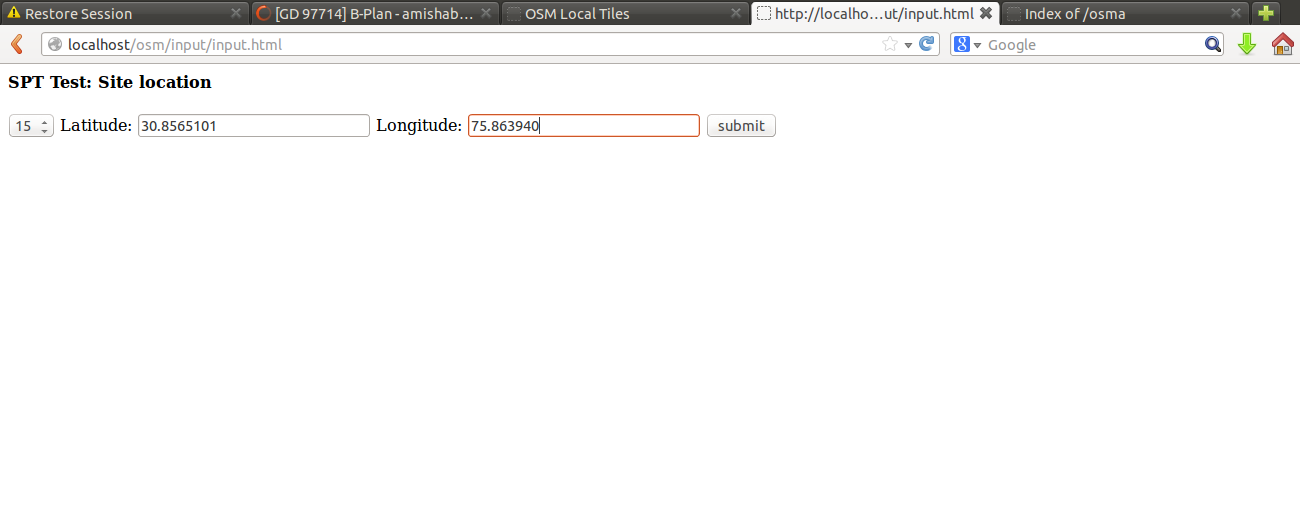
\includegraphics[width=0.7\textwidth]{input/images/osm2.png}
\caption{User Input Page}
\end{figure}

\begin{figure}[h!]
\centering 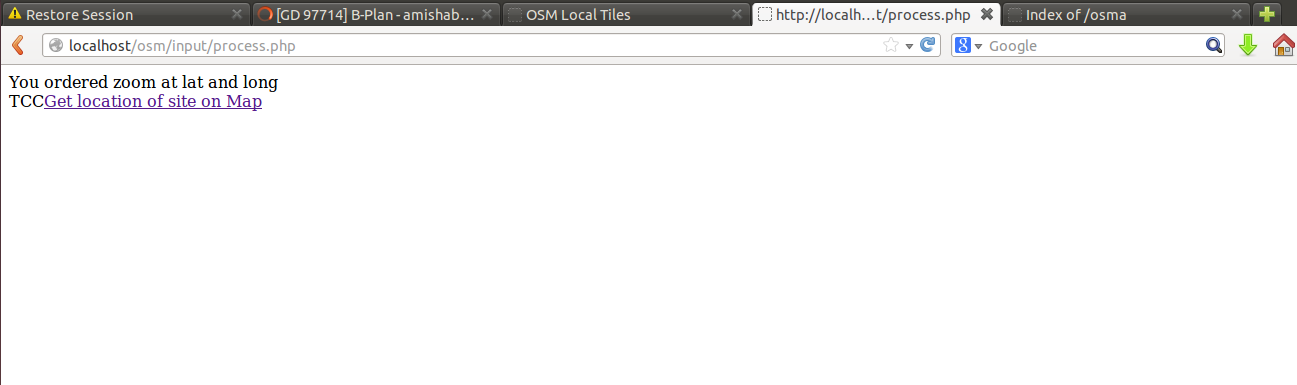
\includegraphics[width=0.7\textwidth]{input/images/osm3.png}
\caption{Php Page}
\end{figure}

\item Phase V (Configurable OSM Installation Script) -: \\
	Building your system as an OSM server, is standalone task that can acquire atleast 15 days for beginner. So the purpose for phase IV is to make a script as easy Wordpress Installation. It is the shell non- interactive, one time configurable script (user have to change hardly two three parameters inside it) at the initial stage and then can run the script and can go for a cup of coffee. The source code of the script is placed under the repository https://github.com/amisha2016/osm\_installation\_script. After running script you will be able to browse to http://your-server-address/osm\_tiles/0/0/0.png as shown below.
\begin{figure}[h!]
	\centering 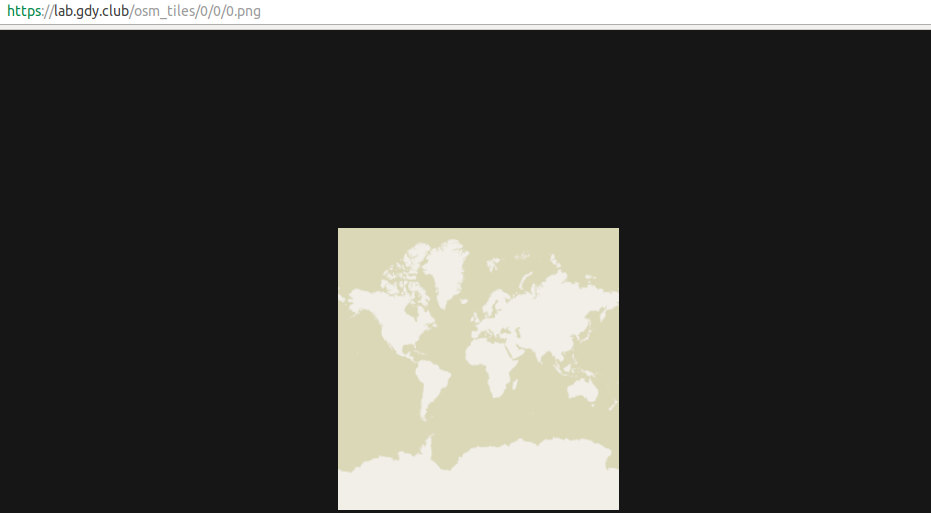
\includegraphics[width=0.7\textwidth]{input/images/osm_script.png}
	\caption{Verifing system to be OSM server using script}
\end{figure}


\item Phase VI (Event Handling) -: \\
The next task was to control the movement of the osm map through the arrow keys of keyboard. Again it is done with the help of Javascript with the concept of event handling. Various formulas are being applied and testing have been done while doing it. The code for the same is on the experimental server. Now, the map can be controlled through arrow keys also. Isn't it amazing?

\item Phase VII (3-D View of the Map) -: \\
The main motive of Phase VII was to make map more realistic. So, by creating the 3-D View of the map it has achieved the greater milestone. It represents OSM Buildings with multiple storyes, shadows of the building, sun, sky and many more. Most of these features are impleented with JOSM tool like creating 3-D tank. The best part of the map is we can tilt and rotate to see a beautiful look.

\begin{figure}[h!]
\centering 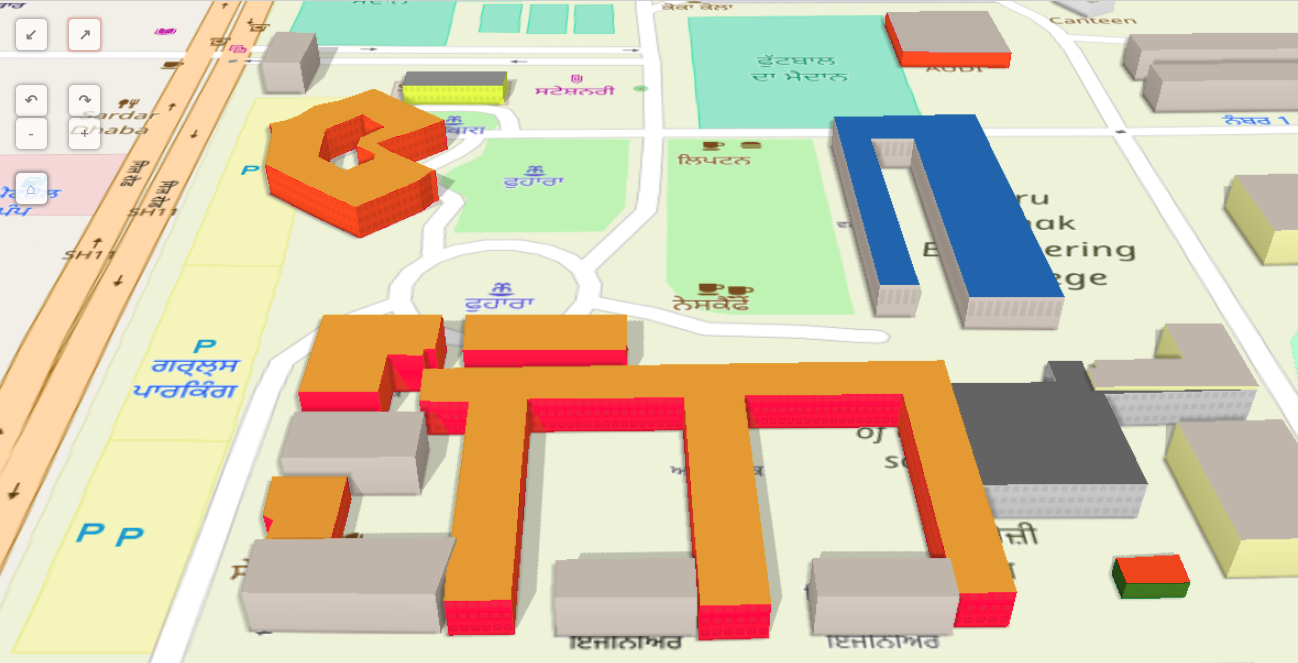
\includegraphics[width=0.7\textwidth]{input/images/osm_building.png}
\caption{Representing 3-D view of GNE}
\end{figure}

\item Phase VIII (Searching the map, Animations, GNE Tour, Popup Menu and Icons) -: \\
	During phase VIII, frontend of the map is improved by adding various features like search button, animations like rotate clockwise, spinning etc. A very beautiful tour of GNE college is represented and the highlighted placed represented by icons. On clicking the map, latitude and longitude is popup.
	\begin{figure}[h!]
		\centering 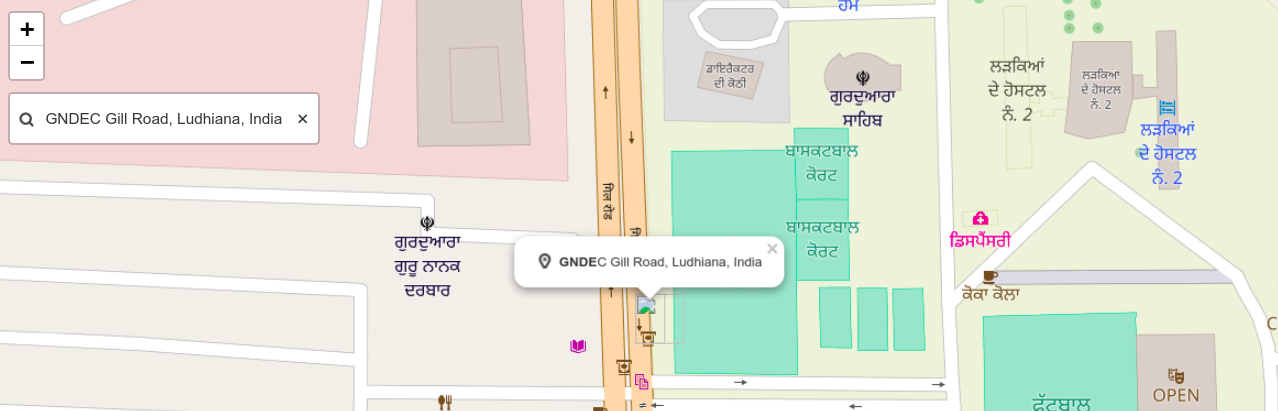
\includegraphics[width=0.7\textwidth]{input/images/osm_search.png}
		\caption{Searched place and pop up menu}
	\end{figure}

        \begin{figure}[h!]
		\centering 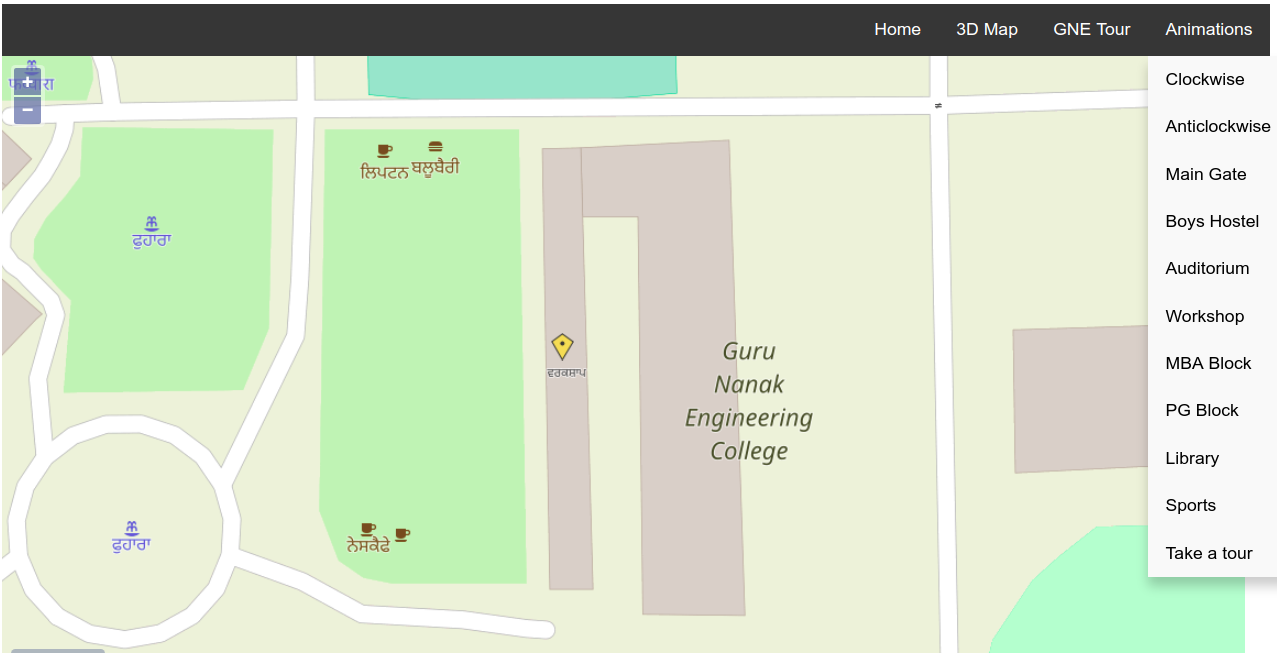
\includegraphics[width=0.7\textwidth]{input/images/osm_animations.png}
		\caption{Representing Animations}
	\end{figure}


\item Phase X (Map On Remote Server) -: \\
All the tasks were achieved on local server first. To make it for others to use for people like you everything is implemented on remote server i.e https://lab.gdy.club. Moreover, it has been kept for back up purpose also so that the code and project retains on other system also.
\begin{figure}[h!]
\centering 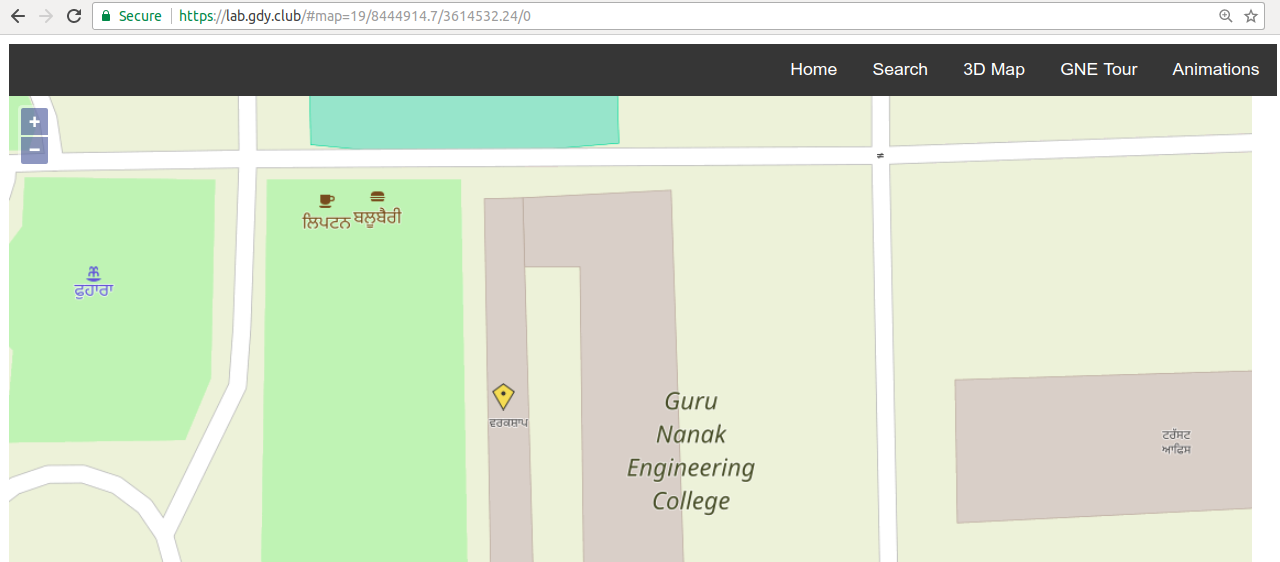
\includegraphics[width=0.7\textwidth]{input/images/osm_remote.png}
\caption{Map on remote server}
\end{figure}

\item Phase XI (Documentation) -: \\
During final phase, the documentation of the project( developers documentation and README.md)
has been made using doxygen and wrote the report in latex for this software.
\end{itemize}

\section{Testing}

